\documentclass[tikz,border=10pt]{standalone}
\usepackage{amsmath}
\usetikzlibrary{calc}

\begin{document}
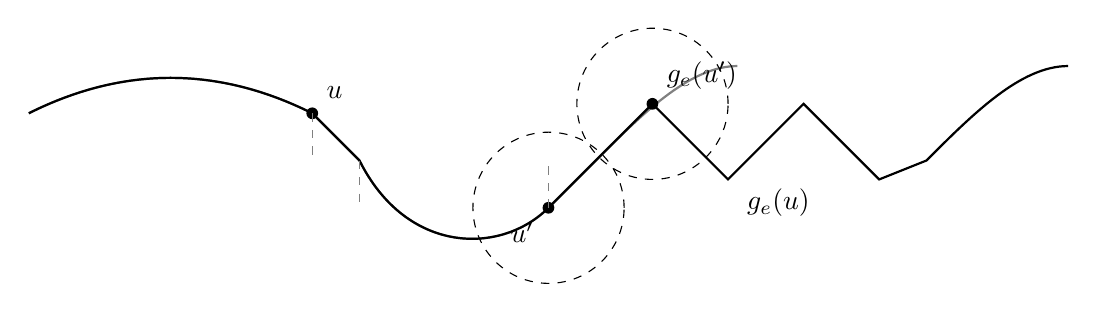
\begin{tikzpicture}[scale=1.2]

% Original Walk (gray)
\draw[thick, gray]
  (-3,1) .. controls (-2,1.5) and (-1,1.5) .. (0,1)
  -- (0.5,0.5) .. controls (1,-0.5) and (2,-0.5) .. (2.5,0)
  -- (3,0.5) .. controls (3.5,1) and (4,1.5) .. (4.5,1.5);

% Modified Walk (black)
\draw[thick, black]
  (-3,1) .. controls (-2,1.5) and (-1,1.5) .. (0,1)
  -- (0.5,0.5) .. controls (1,-0.5) and (2,-0.5) .. (2.5,0)
  -- (3,0.5) .. controls (3.2,0.7) and (3.4,0.9) .. (3.6,1.1)
  -- (3.8,0.9) .. controls (4,0.7) and (4.2,0.5) .. (4.4,0.3)
  -- (4.6,0.5) .. controls (4.8,0.7) and (5,0.9) .. (5.2,1.1)
  -- (5.4,0.9) .. controls (5.6,0.7) and (5.8,0.5) .. (6,0.3)
  -- (6.5,0.5) .. controls (7,1) and (7.5,1.5) .. (8,1.5);

% Points and Labels
\node[circle, fill=black, inner sep=1.5pt, label={above right:$u$}] (u) at (0,1) {};
\node[circle, fill=black, inner sep=1.5pt, label={below left:$u'$}] (uprime) at (2.5,0) {};
\node[circle, fill=black, inner sep=1.5pt, label={above right:$g_e(u')$}] (geuprime) at (3.6,1.1) {};

% Circles around u', g_e(u')
\draw[dashed, thin]
  (uprime) circle (0.8cm);
\draw[dashed, thin]
  (geuprime) circle (0.8cm);

% Additional Labels
\node[below right] at (4.5,0.3) {$g_e(u)$};

% Additional Lines for Clarity
\draw[dashed, gray]
  (0,1) -- (0,0.5);
\draw[dashed, gray]
  (0.5,0.5) -- (0.5,0);
\draw[dashed, gray]
  (2.5,0) -- (2.5,0.5);

\end{tikzpicture}
\end{document}